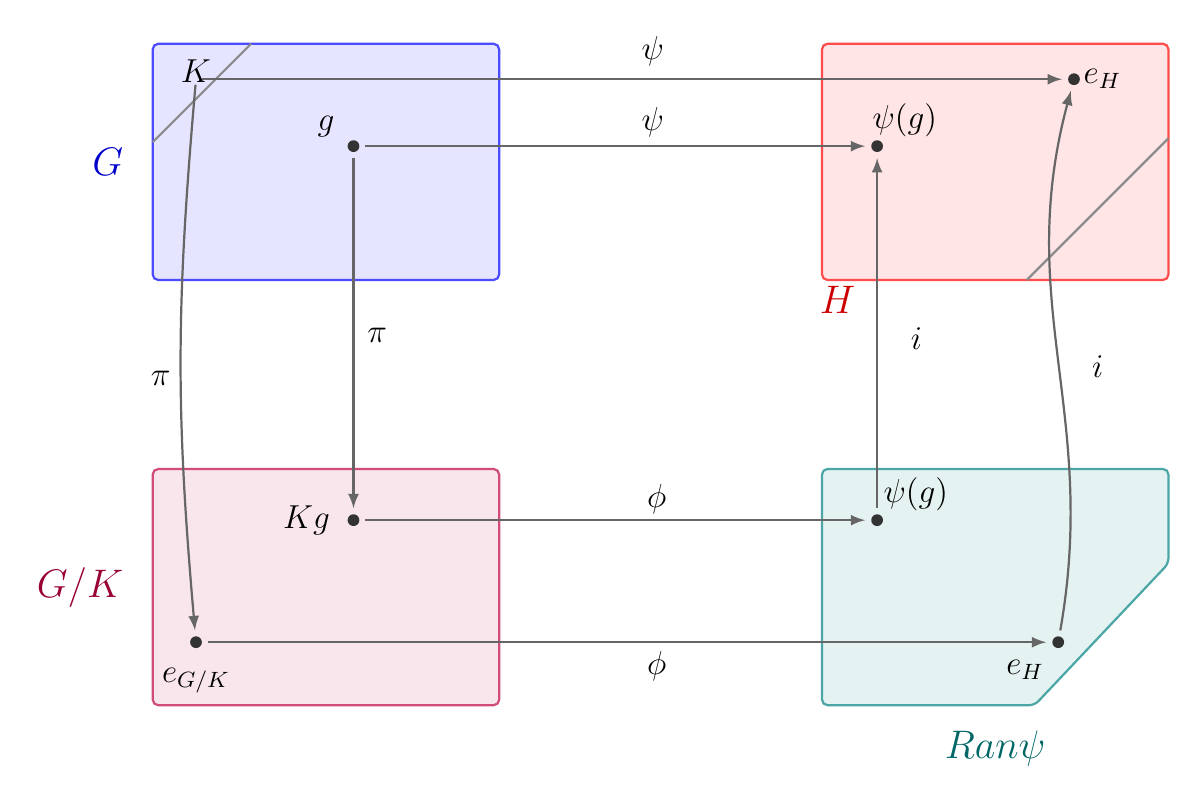
\begin{tikzpicture}[>=latex]

% --- Global TikZ Styles ---
\tikzset{
    setA/.style={fill=blue!10, draw=blue!70, thick, rounded corners=2pt},
    setB/.style={fill=red!10, draw=red!70, thick, rounded corners=2pt},
    setC/.style={fill=purple!10, draw=purple!70, thick, rounded corners=2pt},
    setD/.style={fill=teal!10, draw=teal!70, thick, rounded corners=2pt},
    labelA/.style={text=blue!80!black, font=\Large\bfseries},
    labelB/.style={text=red!80!black, font=\Large\bfseries},
    labelC/.style={text=purple!80!black, font=\Large\bfseries},
    labelD/.style={text=teal!80!black, font=\Large\bfseries},
    point/.style={circle, fill=black!80, inner sep=1.5pt},
    arrow/.style={
        ->,
        >=latex,
        thick,
        draw=black!60,
        shorten >=2pt,
        shorten <=2pt
    },
    innerline/.style={draw=black!45, thick},
    element/.style={font=\large}
}

% ==================================================
% --- Vier verzamelingen / objecten ---
% ==================================================

% --- G linksboven ---
\path[setA] (-2.2, 2.8) rectangle (2.2, 5.8);
\node[labelA, anchor=east] at (-2.45, 4.3) {$G$};
\node[element] at (-1.65, 5.45) {$K$};

% Diagonale lijn in G, zoals in het origineel
\draw[innerline] (-2.2, 4.55) -- (-0.95, 5.8);

% --- H rechtsboven ---
\path[setB] (6.3, 2.8) rectangle (10.7, 5.8);
\node[labelB, anchor=west] at (6.15, 2.55) {$H$};

% Diagonale lijn in H
\draw[innerline] (8.9, 2.8) -- (10.7, 4.6);

% --- G/K linksonder ---
\path[setC] (-2.2, -2.6) rectangle (2.2, 0.4);
\node[labelC, anchor=east] at (-2.45, -1.1) {$G/K$};

% --- Ran psi rechtsonder, met afgesneden hoek ---
\path[setD]
    (6.3, -2.6) --
    (9.0, -2.6) --
    (10.7, -0.8) --
    (10.7, 0.4) --
    (6.3, 0.4) --
    cycle;

\node[labelD] at (8.5, -3.15) {$\operatorname{Ran}\psi$};

% ==================================================
% --- Punten ---
% ==================================================

% Punten in G
\coordinate (K) at (-1.65, 5.35);

\node[point] (g) at (0.35, 4.50) {};
\node[element] at (0.00, 4.75) {$g$};

% Punten in H
\node[point] (psigH) at (7.00, 4.50) {};
\node[element, anchor=south, xshift=10pt] at (psigH) {$\psi(g)$};

\node[point] (eHH) at (9.5, 5.35) {};
\node[element, anchor=west] at (9.5, 5.35) {$e_H$};

% Punten in G/K
\node[point] (Kg) at (0.35, -0.25) {};
\node[element, anchor=east, xshift=-5pt] at (Kg) {$Kg$};

\node[point] (eGK) at (-1.65, -1.80) {};
\node[element, anchor=north] at (-1.65, -2.0) {$e_{G/K}$};

% Punten in Ran psi
\node[point] (psigR) at (7.00, -0.25) {};
\node[element, anchor=south, xshift=14pt] at (psigR) {$\psi(g)$};

\node[point] (eHR) at (9.30, -1.80) {};
\node[element, anchor=north, xshift=-12pt, yshift=-3pt] at (eHR) {$e_H$};

% ==================================================
% --- Pijlen ---
% ==================================================

% psi: G -> H
\draw[arrow] (K) -- (eHH);
\node[element] at (4.15, 5.70) {$\psi$};

\draw[arrow] (g) -- (psigH);
\node[element] at (4.15, 4.8) {$\psi$};

% pi: G -> G/K
\draw[arrow] (K) to[out=-95, in=95, looseness=1.05] (eGK);
\node[element] at (-2.1, 1.55) {$\pi$};

\draw[arrow] (g) -- (Kg);
\node[element] at (0.65, 2.10) {$\pi$};

% phi: G/K -> Ran psi
\draw[arrow] (Kg) -- (psigR);
\node[element] at (4.20, 0.02) {$\phi$};

\draw[arrow] (eGK) -- (eHR);
\node[element] at (4.20, -2.10) {$\phi$};

% i: Ran psi -> H
\draw[arrow] (psigR) -- (psigH);
\node[element] at (7.5, 2.05) {$i$};

\draw[arrow] (eHR) to[out=80, in=-105, looseness=1.05] (eHH);
\node[element] at (9.80, 1.70) {$i$};

\end{tikzpicture}